\subsection{Definition of the \texorpdfstring{$\chi$}{χ} Field}
  \label{subsec:definition-of-the-chi-field}

  We define the existence of a single pre-geometric relational substrate, denoted $\chi$,
  which constitutes the primitive ontological basis of physical reality.
  The quantity $\chi$ is not defined on a pre-existing spacetime manifold and does not
  presuppose any metric, causal, or geometric structure.
  Instead, spacetime notions arise only as effective descriptions of the relational,
  spectral, and dynamical properties of $\chi$ configurations.

  Ontologically, $\chi$ is not a scalar order parameter and does not possess local values.
  Scalar order parameters arise only at the effective level, as coarse-grained descriptors
  of projected $\chi$ configurations once a geometric regime is established.
  Dimensional quantities associated with length, duration, or mass arise only at the
  effective level, when $\chi$ configurations admit a stable geometric interpretation.
  The monotonic ordering intrinsic to $\chi$ configurations gives rise, upon projection,
  to what is operationally perceived as temporal flow.

  \begin{tcolorbox}[colback=white, colframe=blue!75!black, title=Ontological Status of $\chi$]
    The $\chi$ substrate is \textbf{not}:
    \begin{itemize}
      \item A scalar field defined on spacetime (no background manifold).
      \item A discrete lattice or graph.
    \end{itemize}
    It is a \textbf{pre-geometric relational structure} from which spacetime, matter, and
    physical observables emerge through projection.
  \end{tcolorbox}

  Temporal ordering and spatial separation are not fundamental primitives, but arise
  respectively from the intrinsic ordering of $\chi$ configurations and from their
  relational structure once a quasi-stable geometric regime is reached.
  Spatial separation, in turn, arises from relational differences between $\chi$
  configurations, giving rise to an effective notion of distance once a quasi-stable
  geometric regime is reached.
  In this sense, time corresponds to ordering, while space corresponds to relational
  structure.

  The analogy with thermodynamic order parameters applies only at the effective level:
  $\chi$ itself is not an order parameter, but gives rise to effective order parameters
  once projected.
  Within the Cosmochrony framework, $\chi$ therefore provides the minimal ontological
  substrate from which time, space, inertial mass, gravitation, and quantum phenomena
  jointly emerge as harmonics of a single irreversible relaxation process.

  In the following sections, spacetime coordinates, metric quantities, and field-theoretic
  objects will be introduced strictly as effective tools, valid only in regimes where
  $\chi$ admits a stable geometric interpretation.

  \begin{figure}[h]
    \centering
    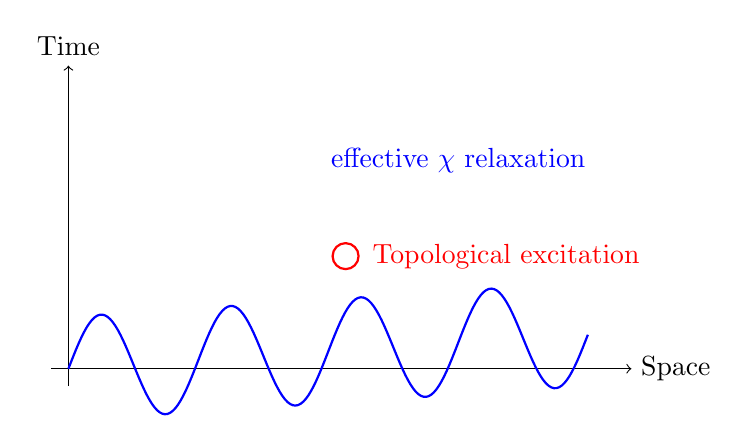
\begin{tikzpicture}[scale=1.1]

% Axes
      \draw[->] (-0.2,0) -- (6.5,0) node[right]{Space};
      \draw[->] (0,-0.2) -- (0,3.5) node[above]{Time};

% Wave
      \draw[thick, blue, domain=0:6, samples=200]
      plot (\x,{0.6*sin(2*pi*\x/1.5 r) + 0.4*\x/6});

% Particle crest
      \draw[red, thick] (3.2,1.3) circle (0.15);
      \node[red, right] at (3.4,1.3) {Topological excitation};

% Annotation
      \node[blue] at (4.5,2.4) {effective $\chi$ relaxation};

    \end{tikzpicture}
    \caption{Conceptual representation of Cosmochrony.
    An effective spacetime depiction of the projected scalar description of $\chi$,
      used for visualization purposes only.
      The monotonic relaxation of $\chi$ gives rise to an effective temporal ordering,
      while localized topological excitations correspond to particle-like configurations
      in the emergent geometric regime.}
    \label{fig:chi_concept}
  \end{figure}

  \paragraph{On the use of spacetime language.}
    Throughout this work, spacetime and field-theoretic language is employed strictly as
    an effective descriptive convenience.
    Such notions refer to emergent, projected constructs that become meaningful only in
    regimes where $\chi$ configurations support a quasi-stable geometric interpretation.
    They do not correspond to fundamental ingredients of the theory.

    Further interpretative clarifications and the fully relational formulation of $\chi$
    are provided in Appendix~\ref{subsec:nature-chi} and
    Appendix~\ref{subsec:relational-configurations-of-chi}.
